\chapter{塑闪阵列探测器的建造}
\label{ch:construction}
相比于地面使用,空间项目对探测器提出了具有更加苛刻的使用条件和更加严格的质量要求。
这不仅意味着要对探测器各部件进行特殊设计以适应火箭发射和空间使用环境,而且探测器的组件生产和整体装配必须遵循一定的建造规范并辅以严格的质量控制程序以保证其达到设计要求和质量。
塑闪阵列探测器的具体设计已经在第\ref{ch:description}章进行了梳理,本章将对它的实际建造过程进行简单介绍。

指导塑闪阵列探测器建造的有两条基本原则:一是要实现其功能要求,二是满足其质量要求。
PSD由探测器主体功能模块,高压扇出模块,前端电子学模块以及机械支撑模块这四部分组成。
其中,高压扇出模块、前端电子学模块和机械支撑模块都由专业的外包单位负责其建造和质量控制,实验室中我们只负责探测器主体功能模块中各探测单元的建造,主要包括是PMT组件以及塑闪单元条组件。
我们还在实验室中将上述四个模块组装成探测器整体,最终完成了塑闪阵列探测器的建造工作。

\section{PMT的筛选}
\label{sec:construction:pmt_selection}
PSD由82个探测单元模块组成,并要求它们之间的MIP能量响应一致性好于$\SI{25}{\percent}$。
PSD探测单元模块的能量响应由PMT的增益以及塑闪单元条的衰减长度共同决定。
由于不同PMT间的个体差异远大于不同塑闪单元条之间的个体差异(见\ref{sec:construction:bar_production}节),选择性能参数相近的PMT显得尤为关键。
因此,我们把PSD中PMT的筛选过程提取出来单独作为一节,对其进行详细描述。

PMT筛选的原理:宇宙线测试参考管子

工厂参数(暗电流与Drift)
去除尺寸和外观检查不合格(光阴极和玻管表面有瑕疵)
去除参与了厂家力学检测

去除极端增益:计算对应于Dy8=700道时的工作电压,去除小于790大于930V的PMT
确定额定工作电压:设定工作电压为810,840,870,900四个档位,分别计算对应的增益,至少有一个电压在600-800之间
选择动态范围:由$1000\cdot Dy58 / Gain$计算额定工作电压下的动态范围,选择$600\sim900$之间的
去除增益随电压变化异常的:计算额定工作电压加90V后的增益相对于原来的比值,选择$1.6\sim 2$之间的

570测试-190挑选焊接-164安装

% 暗电流
PMT的暗电流是指在完全黑暗且没有入射光的条件下,在光电倍增管内部流动的微小电流。
由于暗电流会使得探测器的基线展宽、噪声变大,严重的情况下甚至降低探测器的能量分辨率,因此暗电流越小越好。
光电倍增管的光阴极材料是引起暗电流的主要因素。
PSD采用的R4443型号(即MOD2)使用低噪声的碱金属材料作为光阴极,从而极大地抑制了暗电流的大小。
根据Hamamatsu提供的出厂测试信息,我们发现所有管子的暗电流都小于PSD的要求。
% 增益
R4443的Dy8通道用于覆盖PSD动态范围的低端部分,主要用于$e/\gamma$;R4443的Dy5通道用于覆盖PSD动态范围的高端部分,主要用于相对论重离子的电荷测量。
我们希望Dy8的增益尽量高,使其测得的MIP信号尽量与基线噪声相分离,从而降低$e/\gamma$误判率。
另一方面,PSD对整体的动态范围有严格的区间要求($\SI{0.1}{MIPs}\sim\SI{1400}{MIPs}$),过高的Dy8增益会压低Dy5的增益(即提高了Dy58比值),从而降低Dy5对重离子电荷的分辨能力。
因此

\section{PMT组件的生产}
\label{sec:construction:pmt_production}

\begin{figure}[htbp]
	\centering
	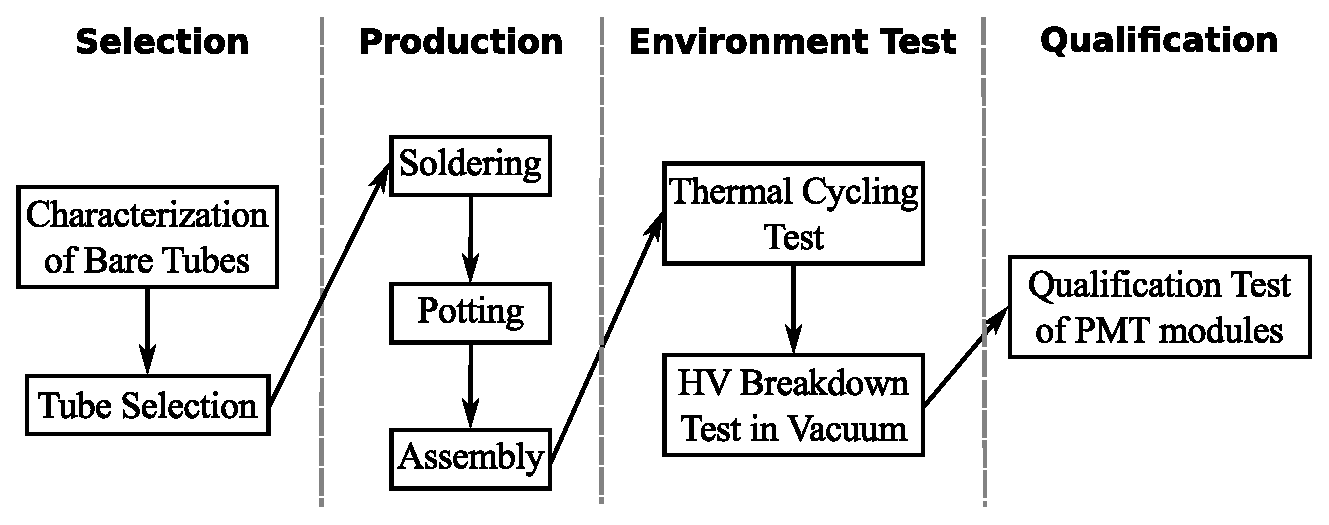
\includegraphics[width=0.95\textwidth]{chap/construction/fig/pmt_production_procedure.eps}
	\caption{PMT组件的生产流程}
	\label{fig:construction:pmt_production_procedure}
\end{figure}

\subsection{结构简介}
\label{sec:construction:pmt_assembly}

\subsection{生产流程}
\label{sec:construction:pmt_procedure}
\begin{enumerate}
	\item PMT的base焊接,信号线+信号头。
	\item 检测:电压、电容。
	\item 灌胶。
	\item 高低温循环。
	\item 真空高压测试。
	\item PMT测试平台测试
\end{enumerate}

\section{塑闪单元条的生产}
\label{sec:construction:bar_production}
测试与筛选过程与PMT正好相反,因为单元条需要包装后才能测试。

\subsection{单元条的包装与测试}
\label{sec:construction:bar_wrapping_and_test}

\subsection{单元条的筛选}
\label{sec:construction:bar_selection}
尺寸复核
热膨胀系数
技术衰减长度:平滑否-包装是否好,两端相差较大也踢出,大于一个值
响应均匀性
探测效率
MPV响应?

\section{探测器整体组装}
\label{sec:construction:psd_assembly}

\subsection{PMT与塑闪单元条的匹配}

\begin{enumerate}
	\item 布单元条。
	\item PMT组件加套筒和播磨合金
	\item 上PMT。
	\item 宇宙线测试。
	\item 上高压扇出板
	\item 上FEE盒子(焊接定位用),上FEE转接板
	\item 上高压接头
	\item 正式上FEE盒子
	\item 上FEE电路板
	\item 上顶板
\end{enumerate}
